\documentclass[10pt,a4paper,twocolumn]{article}
\usepackage[a4paper,top=1.55cm,bottom=1.55cm,left=1.55cm,right=1.55cm,columnsep=0.62cm]{geometry}
\usepackage{fontspec}
\setmainfont{Latin Modern Roman}
\setsansfont{Latin Modern Sans}
\usepackage{microtype}
\usepackage{amsmath}
\usepackage{booktabs}
\usepackage{tabularx}
\usepackage{array}
\usepackage{enumitem}
\usepackage{xcolor}
\usepackage{graphicx}
\usepackage{tikz}
\usetikzlibrary{arrows.meta,positioning,fit,calc}
\usepackage{fancyhdr}
\usepackage{titlesec}
\usepackage{url}
\usepackage{natbib}
\special{pdf:docinfo << /Title (TrustCXR: An Evidence-Governed and Uncertainty-Aware Chest X-ray Research System) /Subject (Frozen Core Research Release) /Keywords (Chest X-ray, Medical Imaging, Deep Learning, Computer Vision, Multi-Label Classification, Predictive Uncertainty, Evidence Verification, Reproducible AI) >>}

\definecolor{ink}{HTML}{172033}
\definecolor{muted}{HTML}{475569}
\definecolor{accent}{HTML}{0F5F78}
\definecolor{rule}{HTML}{CBD5E1}
\definecolor{softblue}{HTML}{E8F1FF}
\definecolor{softpurple}{HTML}{F3E8FF}
\definecolor{softteal}{HTML}{E6FFFA}
\definecolor{softamber}{HTML}{FFF7ED}
\color{ink}
\setlength{\parindent}{1em}
\setlength{\parskip}{0pt}
\setlist{nosep,leftmargin=1.15em}
\titleformat{\section}{\large\bfseries\color{ink}}{\thesection.}{0.35em}{}
\titlespacing*{\section}{0pt}{7pt}{3pt}
\titleformat{\subsection}{\normalsize\bfseries\color{accent}}{\Alph{subsection}.}{0.3em}{}
\titlespacing*{\subsection}{0pt}{4pt}{2pt}
\pagestyle{fancy}
\fancyhf{}
\fancyhead[L]{\footnotesize\textit{TrustCXR: Evidence-Governed Chest X-ray Research}}
\fancyhead[R]{\footnotesize\thepage}
\renewcommand{\headrulewidth}{0.35pt}
\renewcommand{\footrulewidth}{0pt}
\setlength{\headheight}{13pt}
\newcolumntype{Y}{>{\raggedright\arraybackslash}X}
\newcommand{\safeNote}{\vspace{2pt}\noindent\fcolorbox{rule}{gray!5}{\parbox{0.97\columnwidth}{\footnotesize\textit{Research use only. TrustCXR is not a medical diagnostic system and requires expert review.}}}\vspace{3pt}}
\newcommand{\metric}[2]{\textbf{#1} & #2\\}
\newcommand{\tightcaption}[1]{\caption{\small #1}}

\begin{document}
\twocolumn[
\begin{@twocolumnfalse}
\begin{center}
{\LARGE\bfseries TrustCXR: An Evidence-Governed and Uncertainty-Aware Chest X-ray Research System\par}
\vspace{4pt}
{\normalsize Mahmoud Maher El-Said\par}
\vspace{7pt}
\begin{minipage}{0.92\textwidth}
\small
\textbf{Abstract.} Chest X-ray models can produce useful population-level signals while remaining vulnerable to dataset shift, ambiguous labels, and unsupported clinical interpretation. TrustCXR is a frozen, local research system designed around explicit evidence boundaries rather than autonomous diagnosis. The pipeline combines view and technical-quality assessment, a fourteen-label chest-radiograph classifier, model-specific predictive-uncertainty evidence, conservative evidence integration, deterministic research reporting, structured verification, and a defer-first decision policy for expert review. The system preserves provenance and unavailable evidence instead of converting missing support into a positive claim or a contradiction. Frozen internal evaluation of the accepted classifier yielded macro AUROC 0.7287, macro AUPRC 0.1540, and F1 at 0.5 of 0.2072 on 17,061 records from 4,715 patients. These values are research evidence from a governed development/test program, not clinical probabilities or validation of deployment. The release includes bounded local PNG/JPEG inference, a FastAPI service, and a static research interface; it does not include clinical diagnosis, reliable positive lesion localization, external validation, active learning, or language-model reporting.\par
\vspace{3pt}\textbf{Keywords:} chest X-ray; medical imaging; multi-label classification; predictive uncertainty; evidence verification; reproducible AI; expert review
\end{minipage}
\end{center}
\vspace{5pt}
\end{@twocolumnfalse}
]
\safeNote

\section{Introduction}
Chest radiography is widely used for thoracic assessment, and deep learning has made multi-label image classification a practical research direction. Large datasets such as ChestX-ray8/14 and CheXpert enabled learning from weak or uncertain report-derived labels \citep{wang2017chestxray8,irvin2019chexpert}. However, a classifier score alone does not establish a diagnosis, a calibrated clinical probability, or a reliable explanation of where a finding is located. Dataset shift, label semantics, acquisition variation, and incomplete spatial supervision can all make an apparently confident output unsafe to overinterpret.

TrustCXR addresses this systems problem as a research engineering exercise. Its objective is not to automate radiology, but to place a frozen vision pipeline inside an explicit evidence contract: each component has an accepted scope, missing support remains visible, and a deterministic verifier and decision layer can defer a draft when evidence is insufficient. This design is motivated by the broader observation that useful predictive uncertainty is difficult to maintain under distribution shift \citep{ovadia2019uncertainty}.

The contributions of the frozen core are: (1) a patient-governed multi-stage chest X-ray research pipeline; (2) frozen view/quality and fourteen-label classification with model-specific uncertainty evidence; (3) conservative evidence packaging, deterministic report verification, and defer-first research decision support; and (4) a reproducible local application whose unsupported capabilities are explicitly withheld.

\section{Related Work}
Weakly supervised thoracic classification was established at scale by ChestX-ray8, which paired radiographs with report-derived labels and also studied weak localization \citep{wang2017chestxray8}. CheXpert extended this setting with uncertainty labels and expert comparison for selected findings \citep{irvin2019chexpert}. TrustCXR uses these datasets as governed research sources, while preserving their different label semantics rather than treating them as interchangeable ground truth.

The accepted classifier family uses densely connected convolutional representations, a design that promotes feature reuse and short information paths \citep{huang2017densenet}. View/quality and multiview experiments also draw on the practical need to control acquisition context before interpreting a radiograph. For interpretability, Grad-CAM is relevant background for a future attribution study \citep{selvaraju2017gradcam}; it is not implemented in the frozen core, and an attribution map would not by itself establish lesion localization.

\section{Data Governance and Study Design}
Raw datasets remain local and intentionally untracked. Development splits are patient-safe where governed, and locked-test protection is preserved. Dataset roles, label limitations, and external-validation eligibility are summarized in Table~\ref{tab:data}. The accepted classifier evidence uses a frozen internal cohort; no independent external cohort satisfied the release criteria, so external validation was not performed.

\begin{table*}[t]
\centering\small
\caption{Governed dataset roles and final status. Raw images and identifiers are not redistributed.}
\label{tab:data}
\begin{tabularx}{\textwidth}{@{}l l Y Y@{}}
\toprule
\textbf{Dataset} & \textbf{Role} & \textbf{Governance and label scope} & \textbf{Final status}\\
\midrule
NIH ChestX-ray14 & Classification; shared development evidence & Patient-safe split evidence; fourteen dataset-specific labels & Development use; not external\\
CheXmask & Pseudo anatomy evidence & Quality-filtered masks; not lesion ground truth & Limited anatomy research\\
RSNA Pneumonia & Localization baseline & Lung-opacity boxes; narrower than fourteen-label scope & Research baseline only\\
CheXpert Small & View/quality and multiview studies & Different label contract; governed paired splits & Internal experiments; not external\\
Audited candidates & External-validation review & Identity, licensing, or semantics unresolved & No eligible external cohort\\
\bottomrule
\end{tabularx}
\end{table*}

\section{TrustCXR Framework}
\subsection{View and Technical-Quality Assessment}
The perception layer identifies AP, PA, or LATERAL view and produces a non-clinical technical-quality proxy. The proxy is a research control on image usability, not a statement about diagnostic adequacy. On the CheXpert Small internal test, the frozen view head achieved macro F1 0.9861 and the proxy achieved accuracy 0.9994; these values are task-specific and are not compared directly with classifier metrics.

\subsection{Multi-Label Classification}
The frozen classifier returns one research model score for each of the following labels: Atelectasis, Cardiomegaly, Effusion, Infiltration, Mass, Nodule, Pneumonia, Pneumothorax, Consolidation, Edema, Emphysema, Fibrosis, Pleural Thickening, and Hernia. Scores are responses of the model, not calibrated clinical disease probabilities and not diagnoses. The classifier was selected without post-test tuning and retained under a fixed preprocessing and label-order contract.

\subsection{Predictive Uncertainty}
TrustCXR reports predictive uncertainty only where the frozen calibration contract applies. It does not claim epistemic uncertainty, validated out-of-distribution detection, or clinical certainty. This distinction is important because uncertainty quality can degrade under dataset shift even when in-distribution performance appears stable \citep{ovadia2019uncertainty}.

\subsection{Evidence Integration}
Structured outputs are packaged with provenance and scope. Pseudo-anatomy and localization evidence can support limited research statements, but missing spatial evidence is not treated as contradiction. The fusion layer therefore has a maximum partially-supported interpretation and cannot provide reliable positive lesion localization or finding laterality.

\subsection{Deterministic Reporting and Verification}
The report renderer converts structured evidence into a template-bound research draft. A verifier checks claims against accepted structured and provenance evidence, preserving unavailable states and restricting contradiction to explicit governed conflicts. A conservative decision layer applies the precedence DEFER over revise over acceptance for expert review. Acceptance means that a research draft is ready for expert review; it is never clinical approval.

\begin{figure*}[t]
\centering
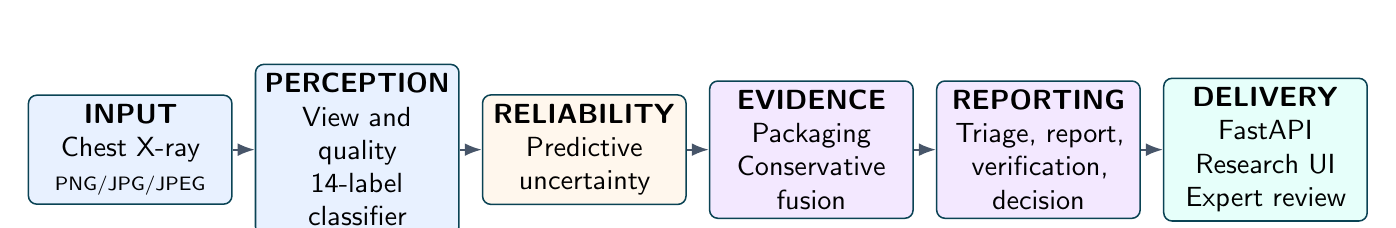
\begin{tikzpicture}[font=\sffamily,>=Latex, node distance=0.28cm]
\tikzset{box/.style={draw=accent!70!black, rounded corners=3pt, minimum height=1.05cm, text width=2.35cm, align=center, fill=softblue, line width=.55pt}, gov/.style={box, fill=softpurple}, del/.style={box, fill=softteal}, rel/.style={box, fill=softamber}, arr/.style={->, line width=.7pt, draw=muted}}
\node[box] (input) {\textbf{INPUT}\\Chest X-ray\\\scriptsize PNG/JPG/JPEG};
\node[box, right=of input] (perc) {\textbf{PERCEPTION}\\View and quality\\14-label classifier};
\node[rel, right=of perc] (unc) {\textbf{RELIABILITY}\\Predictive\\uncertainty};
\node[gov, right=of unc] (evid) {\textbf{EVIDENCE}\\Packaging\\Conservative fusion};
\node[gov, right=of evid] (report) {\textbf{REPORTING}\\Triage, report,\\verification, decision};
\node[del, right=of report] (delivery) {\textbf{DELIVERY}\\FastAPI\\Research UI\\Expert review};
\draw[arr] (input) -- (perc); \draw[arr] (perc) -- (unc); \draw[arr] (unc) -- (evid); \draw[arr] (evid) -- (report); \draw[arr] (report) -- (delivery);
\end{tikzpicture}
\tightcaption{Overview of the frozen TrustCXR research pipeline. Stage identifiers are retained in the release evidence for traceability but are not user-facing capability claims.}
\label{fig:architecture}
\end{figure*}

\section{Experimental Protocol}
The final classifier result was taken from the frozen internal evaluation of 17,061 records from 4,715 patients. Selection was completed on validation evidence, and locked-test records were not re-opened for this paper. Metrics from the separate frontal-only study and the localization baseline are reported with their own cohort qualifications rather than combined into a single ranking. The paper reports existing values only; no metric was recomputed for publication.

\section{Results and Analysis}
Table~\ref{tab:stage9} presents the principal frozen classifier result with sensible display precision. The model provides useful research discrimination evidence, but the modest AUPRC and absence of external validation limit any interpretation beyond the governed cohort.

\begin{table}[t]
\centering\small
\caption{Frozen fourteen-label classifier result. Values are rounded for presentation; full-precision values remain in release evidence.}
\label{tab:stage9}
\begin{tabular}{@{}lr@{}}
\toprule
Metric & Value\\
\midrule
Macro AUROC & 0.7287\\
Macro AUPRC & 0.1540\\
F1 @ 0.5 & 0.2072\\
Test records & 17,061\\
Test patients & 4,715\\
\bottomrule
\end{tabular}
\end{table}

\begin{table*}[t]
\centering\small
\caption{Additional frozen evidence. Cohorts and contracts differ; rows are not superiority comparisons.}
\label{tab:additional}
\begin{tabularx}{\textwidth}{@{}l l l r Y@{}}
\toprule
\textbf{Component} & \textbf{Cohort} & \textbf{Metric} & \textbf{Result} & \textbf{Scientific qualification}\\
\midrule
View assessment & CheXpert Small internal test & Macro F1 & 0.9861 & AP/PA/LATERAL view task\\
Technical-quality proxy & CheXpert Small internal test & Accuracy & 0.9994 & Non-clinical proxy target\\
Pseudo anatomy & NIH CheXmask internal test & Dice / IoU & 0.9714 / 0.9444 & Pseudo anatomy, not lesion ground truth\\
Localization baseline & RSNA validation & Small-lesion sensitivity & 0.0361 & No acceptable operating point\\
Frontal-only classifier & CheXpert exact-pair test & AUROC / AUPRC & 0.8467 / 0.8593 & Different labels/cohort; not comparable to Stage 9\\
\bottomrule
\end{tabularx}
\end{table*}

\section{System Implementation and Reproducibility}
The release provides a local FastAPI service and a static research UI for bounded PNG/JPEG review. The accepted runtime executes the GPU models sequentially, then performs deterministic CPU-side evidence, report, verification, and decision processing. The interface presents current-image model scores and a concise deterministic explanation without an LLM, external requests, browser persistence, or patient workflow.

The reproducibility contract is Windows 11 with Python 3.12.10, PowerShell orchestration, PyTorch cu130, and a governed NVIDIA GPU environment. Seven checkpoint/configuration pairs are retained with SHA-256 evidence. Controlled seeds and frozen configurations support reproducible research execution, but bit-identical CUDA training is not guaranteed. The core release is identified internally as the frozen research release and the UI as the frozen core review interface; these identifiers are implementation traceability, not scientific claims.

\section{Limitations, Ethics, and External Validation}
The system is research use only, is not a medical diagnostic system, and requires expert review. It does not provide treatment recommendations, autonomous clinical release, severity, temporal comparison, or validated OOD detection. The localization baseline has no accepted operating threshold and does not support reliable positive lesion localization; absence of localization must not contradict classifier evidence. Selective prediction was not accepted, and the deterministic triage layer is defer-first.

DICOM interoperability is limited to synthetic/non-patient, single-frame grayscale fixtures under the governed transfer-syntax and photometric contracts. Real-patient DICOM handling and a browser DICOM viewer are outside scope. Human feedback and active learning were withheld because no governed expert-feedback data existed. External validation was not performed because no independent cohort satisfied identity, licensing, label, and cohort-construction requirements. Consequently, the release makes no clinical generalizability, prospective, multi-institutional, or deployment claim.

For release traceability, the frozen evidence disposition is recorded as \texttt{EXTERNAL\_VALIDATION\_NOT\_PERFORMED}; this is an evidence status, not a claim of external evaluation.

Privacy requires that patient identifiers, PHI, raw private DICOM metadata, credentials, and raw datasets remain outside the repository. The project is a reproducible research pipeline, not production clinical MLOps.

\begin{table}[t]
\centering\scriptsize
\caption{Capability and limitation matrix for the frozen core.}
\label{tab:scope}
\begin{tabularx}{\columnwidth}{@{}l l Y@{}}
\toprule
\textbf{Capability} & \textbf{Status} & \textbf{Interpretation}\\
\midrule
Fourteen-label classification & Supported & Frozen research model signals; not diagnoses\\
Predictive uncertainty & Limited & Model-specific predictive evidence only\\
Lesion localization & Withheld & No reliable positive localization or laterality\\
OOD detection & Withheld & Not validated\\
Temporal comparison / severity & Withheld & Not supported\\
DICOM & Limited & Synthetic/non-patient interoperability only\\
External validation & Not performed & No generalizability claim\\
\bottomrule
\end{tabularx}
\end{table}

\section{Future Research Directions}
Post-release work is documented separately and is not implemented in this core paper. A first track may study class-specific visual attribution (for example, Grad-CAM) while describing maps as model attention rather than validated lesion location \citep{selvaraju2017gradcam}. A second track would require independently governed spatial annotations for true pathology localization. A third could evaluate a grounded language model that consumes only structured evidence, keeps the deterministic renderer as a baseline, and remains behind verifier and expert-review gates. A multimodal VLM study would require a separate explicit authorization and comparison against the frozen vision pipeline.

\section{Conclusion}
TrustCXR demonstrates a conservative way to package chest X-ray research models for expert-oriented review. Its contribution is the combination of frozen perception and classification, predictive-uncertainty evidence, provenance-aware evidence handling, deterministic reporting and verification, and a defer-first decision policy within a reproducible local application. The evidence supports a research system with explicit boundaries, not a clinical diagnostic product. External validation, reliable positive localization, active learning, language-model reporting, and other extensions remain future work and are not required for the validity of the frozen core release.

\begingroup\small
\bibliographystyle{unsrtnat}
\bibliography{references}
\endgroup

\section*{Project artifacts}
\small
The frozen manuscript is accompanied by an evidence trail rather than a claim that the paper replaces the underlying records. The final claims matrix, metrics table, dataset-use summary, technical report, reproducibility lock and post-release roadmap remain the authoritative project artifacts. They preserve exact hashes, cohort qualifications, withheld dispositions, and reconstruction instructions without redistributing raw data or patient identifiers.

\begin{table}[b]
\centering\scriptsize
\caption{Selected release artifacts and their role in reproducibility.}
\begin{tabularx}{\columnwidth}{@{}l Y@{}}
\toprule
Artifact & Role\\
\midrule
Claims matrix & Supported, limited, withheld, and prohibited-claim contract\\
Metrics table & Frozen values with cohort and qualification context\\
Dataset-use summary & Governance, split, label, and external-eligibility record\\
Environment lock & Windows/CUDA reconstruction contract\\
Architecture asset & Compact vector description of the frozen core\\
Extension roadmap & Optional, post-release research only; not implemented\\
\bottomrule
\end{tabularx}
\end{table}

\end{document}
